\documentclass[10pt,a4paper]{article}

\usepackage[margin=0.72in]{geometry}
\usepackage{graphicx}
\usepackage{booktabs}
\usepackage{array}
\usepackage{caption}
\usepackage{amsmath}
\usepackage{natbib}
\usepackage[hidelinks]{hyperref}
\usepackage{microtype}

\captionsetup{font=small,labelfont=bf}
\setlength{\parindent}{0pt}
\setlength{\parskip}{4pt}
\setlength{\tabcolsep}{5pt}
\newcommand{\mtt}[1]{\text{\texttt{#1}}}
\newcommand{\githubrepo}{https://github.com/Looloo-dot/ME315-term-life-insurance-q3}

\title{\vspace{-1.5em}\textbf{Household Predictors of Term Life Insurance Coverage}}
\author{ME315 Machine Learning in Practice: Problem Set Day 4, Question 3}
\date{}

\begin{document}
\maketitle
\vspace{-2.0em}

\begin{abstract}
\noindent This paper analyses the Term Life Insurance data set from the 2004 Survey of Consumer Finances to study which household characteristics predict life-insurance coverage. The outcome, the face value of term life insurance, is zero for 225 of 500 households and highly right-skewed among the 275 households with positive coverage. I therefore treat the problem as having two margins: participation, defined by whether coverage is positive, and coverage size, modelled as $\log(\mtt{FACE})$ conditional on positive coverage. The main empirical analysis compares an income-only benchmark, an interpretable OLS model, and regularised Ridge and Lasso specifications. Income, education and household size are the most stable predictors of coverage size. Regularisation improves prediction modestly: across 30 repeated train/test splits, Extended Ridge has the lowest mean test RMSE, followed closely by Lasso. The results support a cautious conclusion: richer models improve predictive performance, but a transparent OLS model remains necessary for substantive interpretation.
\end{abstract}

\section{Introduction}

Life insurance is a household financial product designed to insure against income or wealth loss after the death of an insured person. Economic models of life-cycle behaviour and insurance demand imply that coverage should depend on resources, family responsibilities and demographic characteristics \citep{yaari1965,lewis1989}. Empirical work on life-insurance demand similarly treats income and household structure as central predictors \citep{brownekim1993}. This paper asks a focused empirical question: \emph{which household characteristics are associated with the amount of term life insurance coverage held by a household?}

The analysis is deliberately predictive rather than causal. The aim is not to estimate the causal effect of income or education on insurance purchases, but to use the methods covered so far in ME315 to build a transparent empirical workflow: inspect the data, choose a defensible representation, compare models on held-out data, and interpret the results with appropriate caution. This is important because a model can fit the observed data well while generalising poorly. The paper therefore prioritises out-of-sample performance for model comparison and uses the OLS estimates mainly to explain the direction and size of associations. This framing follows modern empirical machine-learning practice, where results should be reported with a clear evaluation protocol and reproducible code rather than in-sample fit alone \citep{pineau2020}.

\section{Data and empirical strategy}

The data contain 500 households and 18 variables, including demographic characteristics, income, household size, charitable giving, and life-insurance-related variables. The outcome variable is \texttt{FACE}, the amount paid out if the insured party dies. The variable is difficult to model directly: the median is 10,000, the upper quartile is 200,000, and the maximum is 14 million. A key feature of the data is that 225 households have $\mtt{FACE}=0$, while 275 have positive coverage. I therefore distinguish between two related questions: whether a household has any coverage, and how large the coverage is conditional on being positive.

The main analysis models coverage size among households with $\mtt{FACE}>0$. I use $\log(\mtt{FACE})$ as the response because positive \texttt{FACE} is highly right-skewed. Figure~\ref{fig:main}a shows that the log transformation gives a more usable scale for linear modelling. The core predictors are $\log(\mtt{INCOME})$, centred age and age squared, education, household size, the binary gender code, and marital-status dummies. Marital status is dummy-coded because its values are categories, not a continuous scale. The core regression can be read as estimating conditional associations of the form
\[
\log(\mtt{FACE}_i)=\alpha+\beta_1\log(\mtt{INCOME}_i)+X_i'\gamma+\varepsilon_i,
\]
where $X_i$ contains the remaining household covariates. I exclude variables such as \texttt{FACECVLIFEPOLICIES}, \texttt{CASHCVLIFEPOLICIES} and \texttt{BORROWCVLIFEPOL} from the main specification because they are themselves insurance-policy variables. Including them would risk a form of leakage: prediction would be easier, but the model would say less about household characteristics.

Four regression models are compared. The baseline uses only $\log(\mtt{INCOME})$. The core OLS model adds the interpretable demographic and household predictors. Extended Ridge and Extended Lasso use a richer feature set adding log total income, log charitable giving and ethnicity dummies. Ridge shrinks coefficients toward zero, while Lasso can shrink some coefficients exactly to zero; both are useful when richer feature sets may otherwise overfit \citep{hoerlkennard1970,tibshirani1996}. The main split assigns 75 percent of positive-coverage households to training and 25 percent to testing. Ridge and Lasso are fitted with standardisation and cross-validated penalty choices using the training data. Performance is measured by RMSE on held-out test data. Because a single split can be noisy in a sample of 275 positive-coverage households, I also repeat the train/test evaluation over 30 random splits. For coefficient interpretation, I estimate the core OLS model on the full positive-coverage sample using HC3 robust standard errors.

\begin{figure}[t]
\centering
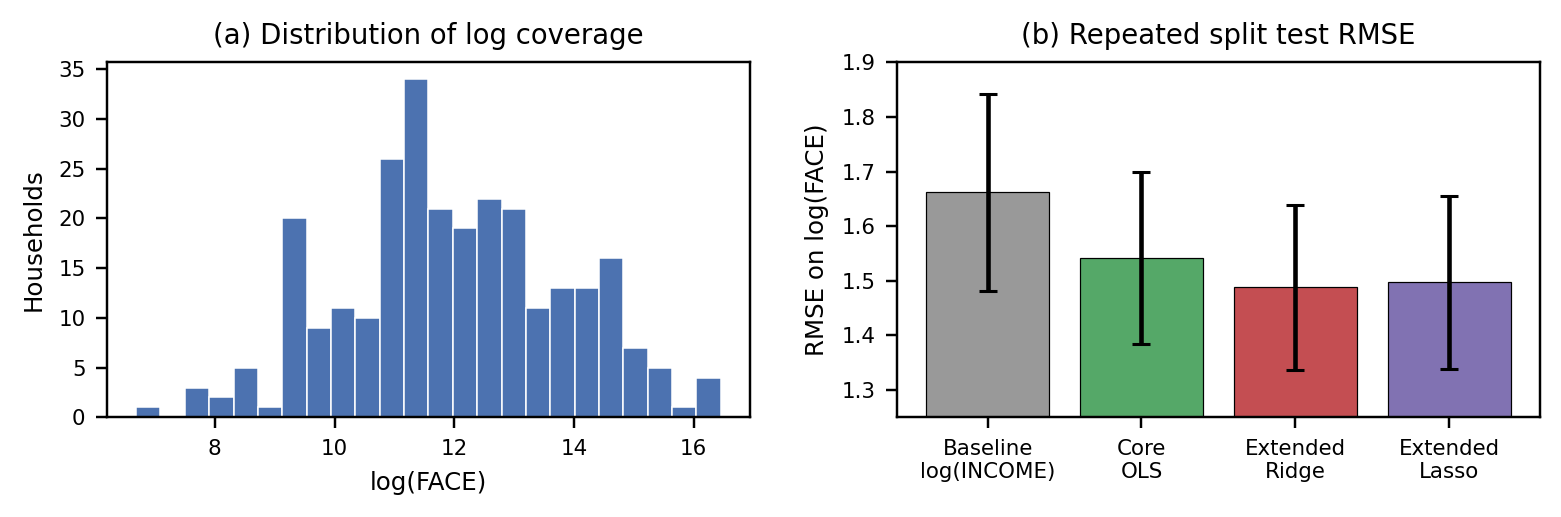
\includegraphics[width=0.94\linewidth]{figures/figure1_distribution_model_comparison.png}
\caption{Outcome representation and predictive comparison. Panel (a) shows the distribution of $\log(\mtt{FACE})$ among households with positive coverage. Panel (b) reports repeated train/test RMSE means with one standard deviation across 30 random splits.}
\label{fig:main}
\end{figure}

\section{Results}

Table~\ref{tab:ols} reports the full-sample robust OLS estimates for the core model. Income is positively associated with coverage size: the coefficient on $\log(\mtt{INCOME})$ is 0.412, so a 1 percent increase in income is associated with about a 0.41 percent increase in coverage, conditional on the other variables. Education is also strongly positive, and household size is positive, consistent with the interpretation that larger households may have greater insurance needs. The binary gender-code coefficient is positive in this specification, although the dataset does not itself make this a causal gender effect. Age and marital status are not precisely estimated. These are conditional associations, not causal effects.

\begin{table}[h]
\centering
\caption{Core OLS model for $\log(\mtt{FACE})$ among positive-coverage households}
\label{tab:ols}
\begin{tabular}{lrrr}
\toprule
Variable & Coef. & Robust s.e. & $p$-value \\
\midrule
$\log(\mtt{INCOME})$ & 0.412 & 0.121 & 0.001 \\
Age $-50$ & -0.010 & 0.008 & 0.252 \\
$(\text{Age}-50)^2$ & -0.001 & 0.000 & 0.055 \\
Education & 0.213 & 0.044 & $<0.001$ \\
Household size & 0.206 & 0.071 & 0.004 \\
Gender & 0.701 & 0.326 & 0.032 \\
Married & 0.228 & 0.331 & 0.491 \\
Living with partner & -0.608 & 0.624 & 0.330 \\
\bottomrule
\end{tabular}
\caption*{\footnotesize Notes: $N=275$ positive-coverage households. The omitted marital-status category is \texttt{MARSTAT}=0. Standard errors are HC3 robust. The model has $R^2=0.376$ and adjusted $R^2=0.357$.}
\end{table}

Table~\ref{tab:pred} compares predictive performance. On the main split, the income-only benchmark has test RMSE 1.587. The core OLS model improves this to 1.448. Extended Ridge gives the lowest test RMSE, 1.438, while Extended Lasso is essentially tied at 1.449. The repeated-split results are more informative: Ridge has the lowest mean test RMSE, 1.488, followed by Lasso at 1.497, core OLS at 1.542 and the baseline at 1.662. Ridge is best in 18 of the 30 splits, Lasso in 8, core OLS in 3 and the baseline in 1. Since RMSE is measured in log points, these results should be interpreted as relative predictive accuracy on the transformed coverage scale rather than average dollar error.

\begin{table}[h]
\centering
\caption{Predictive performance for $\log(\mtt{FACE})$}
\label{tab:pred}
\begin{tabular}{lrrr}
\toprule
Model & Main test RMSE & Repeated-split RMSE & Mean test $R^2$ \\
\midrule
Baseline: $\log(\mtt{INCOME})$ & 1.587 & 1.662 & 0.168 \\
Core OLS & 1.448 & 1.542 & 0.287 \\
Extended Ridge & 1.438 & 1.488 & 0.338 \\
Extended Lasso & 1.449 & 1.497 & 0.329 \\
\bottomrule
\end{tabular}
\caption*{\footnotesize Notes: The main split uses a 75/25 train/test split of positive-coverage households. Repeated-split RMSE and mean test $R^2$ are averages across 30 random splits.}
\end{table}

These differences should not be overstated. Ridge is the strongest predictive model, but the improvement over Lasso and core OLS is moderate. The best interpretation is that regularisation helps when extra predictors are added, while the core OLS model remains useful for explaining which variables matter. A short classification extension predicts whether $\mtt{FACE}>0$. Lasso logistic performs best among the tested classifiers, with accuracy 0.664, F1 score 0.708, AUC 0.707 and log loss 0.636. This confirms that participation is a distinct empirical margin, although it is secondary to the main coverage-size analysis. It also reinforces the central modelling decision: treating zero coverage and positive coverage as the same continuous outcome would blur two different household decisions.

\section{Conclusion}

The main empirical finding is that income, education and household size are the clearest predictors of term life insurance coverage among households with positive coverage. The modelling exercise also shows why careful representation matters: raw coverage is too skewed for a simple linear model, and the zero values imply a separate participation question. Regularised methods modestly improve prediction, especially Ridge, but the interpretable OLS model remains competitive and easier to communicate.

The analysis has limitations. The data are observational, so the estimates should not be read causally. The positive-coverage sample has only 275 observations, so model rankings are not perfectly stable. Finally, I exclude policy-specific variables to avoid leakage, which improves interpretability but limits predictive power. Even with these limitations, the exercise provides a rigorous template for the final project: define a precise empirical question, justify feature choices, compare models using held-out performance, and report results in a reproducible workflow.

\small
\begin{thebibliography}{9}
\bibitem[Browne and Kim(1993)]{brownekim1993}
Browne, M. J. and Kim, K. (1993).
An international analysis of life insurance demand.
\emph{Journal of Risk and Insurance}, 60(4), 616--634.

\bibitem[Lewis(1989)]{lewis1989}
Lewis, F. D. (1989).
Dependents and the demand for life insurance.
\emph{American Economic Review}, 79(3), 452--467.

\bibitem[Hoerl and Kennard(1970)]{hoerlkennard1970}
Hoerl, A. E. and Kennard, R. W. (1970).
Ridge regression: biased estimation for nonorthogonal problems.
\emph{Technometrics}, 12(1), 55--67.

\bibitem[Pineau et al.(2020)]{pineau2020}
Pineau, J., Vincent-Lamarre, P., Sinha, K., Lariviere, V., Beygelzimer, A., Fox, E. and Larochelle, H. (2020).
Improving reproducibility in machine learning research.
\emph{arXiv:2003.12206}.

\bibitem[Tibshirani(1996)]{tibshirani1996}
Tibshirani, R. (1996).
Regression shrinkage and selection via the lasso.
\emph{Journal of the Royal Statistical Society: Series B}, 58(1), 267--288.

\bibitem[Yaari(1965)]{yaari1965}
Yaari, M. E. (1965).
Uncertain lifetime, life insurance, and the theory of the consumer.
\emph{Review of Economic Studies}, 32(2), 137--150.
\end{thebibliography}

\clearpage
\normalsize
\appendix
\section*{Appendix}

\subsection*{A.1 Files Required to Reproduce the Analysis}

\begin{table}[h]
\centering
\footnotesize
\caption*{Appendix Table A1. Submission files}
\begin{tabular}{>{\raggedright\arraybackslash\ttfamily}p{0.30\linewidth}>{\raggedright\arraybackslash}p{0.62\linewidth}}
\toprule
\normalfont File & \normalfont Purpose \\
\midrule
Q3 notebook.ipynb & Main empirical notebook containing data inspection, feature construction, model fitting, robustness checks and classification extension. \\
Term Life Insurance.csv & Dataset used by the notebook. It should remain in the same folder as the notebook so the relative file path works. \\
term\_life\_q3\_report.tex & LaTeX source for the written report and appendix. \\
figures/figure1\_\allowbreak distribution\_\allowbreak model\_\allowbreak comparison.png & Figure used in the report, showing the transformed outcome and repeated-split model comparison. \\
ProblemSetDay04.pdf & Original problem-set document. \\
\bottomrule
\end{tabular}
\end{table}

\subsection*{A.2 GitHub Repository Links}

For transparency, the empirical materials are stored together in the GitHub repository
\begin{center}
\href{https://github.com/Looloo-dot/term-life-insurance}{\texttt{Looloo-dot/term-life-insurance}}.
\end{center}
The key files are linked below:
\begin{itemize}
\item Dataset: \href{https://github.com/Looloo-dot/term-life-insurance/blob/main/Term\%20Life\%20Insurance.csv}{\texttt{Term Life Insurance.csv}}
\item Jupyter notebook: \href{https://github.com/Looloo-dot/term-life-insurance/blob/main/Q3\%20notebook.ipynb}{\texttt{Q3 notebook.ipynb}}
\item Figure: \href{https://github.com/Looloo-dot/term-life-insurance/blob/main/figures/figure1\_distribution\_model\_comparison.png}{\texttt{figure1\_\allowbreak distribution\_\allowbreak model\_\allowbreak comparison.png}}
\item LaTeX report source: \href{https://github.com/Looloo-dot/term-life-insurance/blob/main/term\_life\_q3\_report.tex}{\texttt{term\_life\_q3\_report.tex}}
\end{itemize}

\subsection*{A.3 Reproducibility Instructions}

The notebook is designed to be run from the submission folder. The data are loaded with the relative path
\[
\texttt{pd.read\_csv("Term Life Insurance.csv")}.
\]
Therefore, the dataset should be uploaded to the same GitHub or Overleaf-linked project folder as the notebook. The empirical analysis uses Python with \texttt{pandas}, \texttt{numpy}, \texttt{matplotlib}, \texttt{statsmodels} and \texttt{scikit-learn}. The main regression split uses \texttt{random\_state=123}; the repeated-split robustness check uses seeds 100 to 129. These fixed seeds make the reported model comparisons reproducible.

\subsection*{A.4 Empirical Decisions}

The main outcome, \texttt{FACE}, has many zero values and a highly skewed positive distribution. For this reason, the report separates the analysis into a participation margin, whether $\mtt{FACE}>0$, and a coverage-size margin, $\log(\mtt{FACE})$ conditional on positive coverage. The latter is the main empirical exercise because it directly studies the amount of coverage held by insured households.

The main predictors are household characteristics available before observing policy size: income, age, education, household size, gender code and marital status. Policy-specific variables such as \texttt{FACECVLIFEPOLICIES}, \texttt{CASHCVLIFEPOLICIES} and \texttt{BORROWCVLIFEPOL} are excluded from the main models because they are too mechanically related to insurance holdings. This avoids leakage and keeps the analysis focused on household-level predictors.

\subsection*{A.5 Course Methods Used}

Data inspection, transformations and feature engineering motivate the log outcome and dummy variables. Train/test evaluation and RMSE are used for predictive comparison. Ridge and Lasso are used to assess whether regularisation improves prediction when the feature set is expanded. Logistic regression and classification metrics are used only as a short extension for the participation margin.

\subsection*{A.6 Interpretation Boundaries}

The estimates are observational associations. They should not be interpreted as causal effects of income, education, gender or household size on insurance demand. The sample of positive-coverage households contains 275 observations, so model rankings are informative but not definitive. The repeated-split results are included precisely to avoid relying too heavily on one favourable train/test split.

\end{document}
